\mode*
\mode<all>{\topsection{Krzywe w $\R^3$}}

\begin{frame}[<+->]
\begin{center}
%\Large Krzywe w $\R^3$.\\[0.2in]
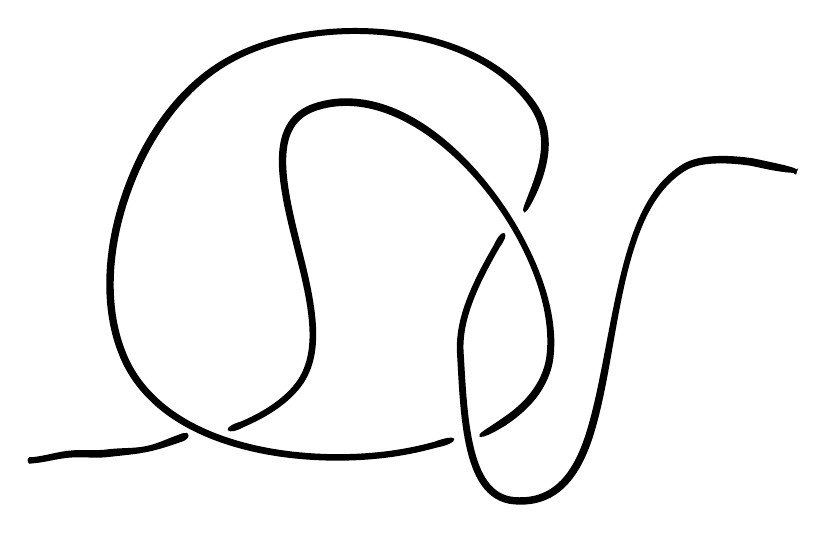
\begin{tikzpicture}[y=0.80pt, x=0.8pt,scale=0.7,yscale=-1, inner sep=0pt, outer sep=0pt]
\begin{scope}[shift={(69.41462,-293.94043)}]% layer1
  % path848
  \path[draw=black,fill=black,line cap=round,miter limit=4.00,line width=0.880pt]
    (30.6103,555.9949) .. controls (26.7121,557.2762) and (22.8747,558.9172) ..
    (18.9822,560.4516) .. controls (15.0898,561.9861) and (11.1433,563.4136) ..
    (7.0880,564.2563) .. controls (3.0327,565.0990) and (-1.1218,565.3550) ..
    (-5.2732,565.5354) .. controls (-9.4247,565.7158) and (-13.5740,565.8210) ..
    (-17.6729,566.3700) .. controls (-23.7136,567.1791) and (-29.8765,566.7917) ..
    (-35.9714,566.8653) .. controls (-38.1470,566.8912) and (-40.3156,566.9750) ..
    (-42.4749,567.1912) .. controls (-48.1963,567.7639) and (-53.8666,569.2667) ..
    (-59.5911,570.3752) .. controls (-59.5911,570.3752) and (-59.5911,570.3752) ..
    (-59.5911,570.3752) .. controls (-61.8264,570.8080) and (-64.0683,571.1807) ..
    (-66.3179,571.4064) .. controls (-66.5706,571.4318) and (-66.8235,571.4553) ..
    (-67.0766,571.4767) .. controls (-67.5104,571.2683) and (-67.8535,571.2713) ..
    (-68.1122,571.4053) .. controls (-68.3164,571.5110) and (-68.4684,571.6983) ..
    (-68.5697,571.9275) -- (-68.5697,571.9275) -- (-68.5697,571.9275) .. controls
    (-68.6211,572.0437) and (-68.6595,572.1708) .. (-68.6850,572.3034) .. controls
    (-68.6850,572.3034) and (-68.6850,572.3034) .. (-68.6850,572.3034) .. controls
    (-68.6978,572.3702) and (-68.7073,572.4384) .. (-68.7136,572.5073) .. controls
    (-68.7136,572.5073) and (-68.7136,572.5073) .. (-68.7136,572.5073) .. controls
    (-68.7266,572.6516) and (-68.7252,572.7992) .. (-68.7094,572.9439) .. controls
    (-68.7018,573.0135) and (-68.6908,573.0825) .. (-68.6765,573.1501) .. controls
    (-68.6765,573.1501) and (-68.6765,573.1501) .. (-68.6765,573.1501) .. controls
    (-68.6480,573.2851) and (-68.6062,573.4148) .. (-68.5519,573.5335) --
    (-68.5519,573.5335) -- (-68.5519,573.5335) -- (-68.5519,573.5335) .. controls
    (-68.4428,573.7706) and (-68.2817,573.9641) .. (-68.0732,574.0705) --
    (-68.0732,574.0705) .. controls (-67.7901,574.2151) and (-67.4164,574.1989) ..
    (-66.9621,573.9124) .. controls (-66.7289,573.8974) and (-66.4961,573.8806) ..
    (-66.2637,573.8623) .. controls (-63.9965,573.6836) and (-61.7390,573.3553) ..
    (-59.4909,572.9660) .. controls (-59.4909,572.9660) and (-59.4909,572.9660) ..
    (-59.4909,572.9660) .. controls (-53.7865,571.9781) and (-48.1334,570.5973) ..
    (-42.4286,570.1409) .. controls (-40.2020,569.9627) and (-37.9652,569.9252) ..
    (-35.7212,569.9456) .. controls (-29.7179,570.0006) and (-23.6451,570.4763) ..
    (-17.6875,569.7679) .. controls (-9.5030,568.7947) and (-0.4832,568.1299) ..
    (7.5931,566.4802) .. controls (15.6695,564.8305) and (22.7637,562.2629) ..
    (30.5394,559.6359) .. controls (31.9415,559.0797) and (34.6129,557.0867) ..
    (32.9860,555.7526) .. controls (32.2094,555.4988) and (31.3681,555.7904) ..
    (30.6103,555.9949) -- cycle(236.5726,550.6302) .. controls (242.9665,546.6485)
    and (248.9511,541.9679) .. (254.1551,536.4444) .. controls (254.1551,536.4444)
    and (254.1551,536.4444) .. (254.1551,536.4444) .. controls (262.1196,528.0020)
    and (267.7930,517.2089) .. (269.0633,505.7013) .. controls (269.0633,505.7013)
    and (269.0633,505.7013) .. (269.0633,505.7013) .. controls (270.1123,495.8517)
    and (269.2990,485.9655) .. (267.3853,476.4043) .. controls (265.2853,465.9030)
    and (261.8736,455.7443) .. (257.6802,445.9663) .. controls (255.1715,440.1168)
    and (252.3928,434.3943) .. (249.3767,428.8006) .. controls (241.5584,414.3009)
    and (232.1375,400.6460) .. (221.3367,388.1567) .. controls (213.9888,379.6600)
    and (205.9572,371.7140) .. (197.1563,364.6659) .. controls (197.1563,364.6659)
    and (197.1563,364.6659) .. (197.1563,364.6659) .. controls (188.9439,358.0882)
    and (180.0410,352.2782) .. (170.4259,347.8667) .. controls (164.0621,344.9453)
    and (157.3616,342.6481) .. (150.4689,341.3006) .. controls (147.8551,340.7897)
    and (145.2167,340.4019) .. (142.5586,340.1543) .. controls (133.3683,339.3001)
    and (123.9703,340.2363) .. (115.1885,343.2704) .. controls (111.8565,344.4200)
    and (108.6360,346.0208) .. (105.7684,348.1863) .. controls (103.2031,350.1293)
    and (100.9715,352.5197) .. (99.2071,355.2349) .. controls (97.4351,357.9703)
    and (96.1422,360.9799) .. (95.2532,364.0772) .. controls (94.2855,367.4453)
    and (93.7594,370.9066) .. (93.5188,374.3520) .. controls (92.9606,382.3671)
    and (93.7734,390.3656) .. (95.0062,398.1586) .. controls (95.0062,398.1586)
    and (95.0062,398.1586) .. (95.0062,398.1586) .. controls (96.4199,407.1545)
    and (98.4367,416.0051) .. (100.5659,424.7668) .. controls (100.5659,424.7668)
    and (100.5659,424.7668) .. (100.5659,424.7668) .. controls (101.4450,428.3951)
    and (102.3568,432.0127) .. (103.2725,435.6229) .. controls (106.9300,450.0414)
    and (110.6492,464.3283) .. (112.3475,478.9370) .. controls (113.2804,486.9927)
    and (113.5937,495.1398) .. (112.2960,503.1073) .. controls (111.1190,510.3269)
    and (108.4898,517.4139) .. (103.9938,523.2688) .. controls (103.9938,523.2688)
    and (103.9938,523.2688) .. (103.9938,523.2688) .. controls (99.0173,529.7576)
    and (92.5146,535.0432) .. (85.5403,539.4426) .. controls (85.5403,539.4426)
    and (85.5403,539.4426) .. (85.5403,539.4426) .. controls (80.1180,542.8643)
    and (74.3839,545.7783) .. (68.4860,548.3106) .. controls (65.4838,549.2442)
    and (63.3762,550.1321) .. (62.0714,550.9136) .. controls (60.7666,551.6952)
    and (60.2667,552.3655) .. (60.4923,552.7744) .. controls (60.7178,553.1833)
    and (61.6711,553.3299) .. (63.2568,553.0124) .. controls (64.8425,552.6950)
    and (67.0660,551.9128) .. (69.7620,550.4210) .. controls (75.6391,547.9074)
    and (81.3766,545.0058) .. (86.8359,541.5964) .. controls (86.8359,541.5964)
    and (86.8359,541.5964) .. (86.8359,541.5964) .. controls (93.9997,537.1374)
    and (100.7417,531.6853) .. (106.0122,524.9124) .. controls (106.0122,524.9124)
    and (106.0122,524.9124) .. (106.0122,524.9124) .. controls (110.8374,518.6562)
    and (113.6755,511.1903) .. (114.9293,503.6179) .. controls (116.3080,495.3037)
    and (116.0381,486.9006) .. (115.1073,478.6895) .. controls (113.4581,464.1048)
    and (109.8819,449.9325) .. (106.3466,435.7635) .. controls (105.3729,431.8611)
    and (104.4025,427.9601) .. (103.4713,424.0564) .. controls (103.4713,424.0564)
    and (103.4713,424.0564) .. (103.4713,424.0564) .. controls (101.3831,415.2974)
    and (99.4167,406.5077) .. (98.0626,397.6372) .. controls (98.0626,397.6372)
    and (98.0626,397.6372) .. (98.0626,397.6372) .. controls (96.8903,389.9384)
    and (96.1206,382.1670) .. (96.7024,374.5220) .. controls (96.9514,371.2455)
    and (97.4537,368.0068) .. (98.3644,364.9163) .. controls (99.2004,362.0823)
    and (100.3754,359.3682) .. (101.9628,356.9612) .. controls (103.5306,354.5749)
    and (105.5168,352.4708) .. (107.7869,350.7699) .. controls (110.3267,348.8584)
    and (113.2477,347.4337) .. (116.3097,346.3801) .. controls (116.3097,346.3801)
    and (116.3097,346.3801) .. (116.3097,346.3801) .. controls (124.5955,343.5364)
    and (133.5151,342.6814) .. (142.2518,343.4997) .. controls (144.0997,343.6719)
    and (145.9406,343.9168) .. (147.7726,344.2278) .. controls (154.9780,345.4511)
    and (162.1487,347.7999) .. (169.0538,350.9175) .. controls (178.3076,355.1009)
    and (187.0851,360.6829) .. (195.2843,367.0831) .. controls (195.2843,367.0831)
    and (195.2843,367.0831) .. (195.2843,367.0832) .. controls (203.9952,373.8867)
    and (212.0379,381.6260) .. (219.3771,389.9033) .. controls (230.5414,402.5034)
    and (240.1207,416.2992) .. (247.7006,430.5023) .. controls (250.5787,435.8952)
    and (253.1747,441.3460) .. (255.4909,446.8561) .. controls (259.6116,456.6638)
    and (262.8206,466.6565) .. (264.7283,476.8510) .. controls (266.4814,486.2394)
    and (267.1545,495.8112) .. (266.0291,505.2756) .. controls (264.7981,515.8764)
    and (259.4144,525.9649) .. (251.7450,534.0648) .. controls (247.9123,538.1116)
    and (243.5794,541.7328) .. (238.8770,544.9913) .. controls (237.2214,546.1625)
    and (235.1076,547.6317) .. (232.9283,549.0881) .. controls (230.7489,550.5444)
    and (228.5067,551.9895) .. (226.6743,553.2149) .. controls (224.8419,554.4403)
    and (223.4232,555.4525) .. (222.9137,556.0836) .. controls (222.4041,556.7147)
    and (222.8060,556.9779) .. (224.5999,556.6052) .. controls (228.3233,555.3435)
    and (232.7670,552.9500) .. (236.5727,550.6302) -- cycle(260.5022,394.4476) ..
    controls (262.6697,388.8067) and (264.3778,382.9603) .. (265.3112,376.8955) ..
    controls (266.1757,371.2225) and (266.2227,365.3557) .. (265.1211,359.6350) ..
    controls (265.1211,359.6350) and (265.1211,359.6350) .. (265.1211,359.6350) ..
    controls (263.9653,353.7224) and (261.5591,348.1362) .. (258.2299,343.2261) ..
    controls (258.2299,343.2261) and (258.2299,343.2261) .. (258.2299,343.2261) ..
    controls (248.2160,328.5104) and (233.6791,317.5848) .. (217.9227,310.1086) ..
    controls (200.8060,301.9802) and (182.2118,297.5422) .. (163.5076,295.6104) ..
    controls (157.5079,294.9909) and (151.4837,294.6290) .. (145.4565,294.5232) ..
    controls (132.1595,294.2898) and (118.8443,295.3018) .. (105.7490,297.6518) ..
    controls (88.0223,300.8341) and (70.5474,306.4629) .. (55.1052,315.9080) ..
    controls (55.1052,315.9080) and (55.1052,315.9080) .. (55.1052,315.9080) ..
    controls (40.0417,325.1275) and (27.2970,337.9294) .. (16.9437,352.2829) ..
    controls (10.9170,360.6336) and (5.6648,369.5381) .. (1.2265,378.8321) ..
    controls (-2.4676,386.5679) and (-5.6734,394.5373) .. (-8.3801,402.6695) ..
    controls (-14.2849,420.3994) and (-17.8504,439.0125) .. (-18.0092,457.8034) ..
    controls (-18.0092,457.8034) and (-18.0092,457.8034) .. (-18.0092,457.8034) ..
    controls (-18.1651,475.3553) and (-15.2115,493.2091) .. (-7.6598,509.3036) ..
    controls (-7.6598,509.3036) and (-7.6598,509.3036) .. (-7.6598,509.3036) ..
    controls (-1.2929,522.7890) and (8.9389,534.2037) .. (20.9350,542.8701) ..
    controls (20.9350,542.8701) and (20.9350,542.8701) .. (20.9350,542.8701) ..
    controls (21.1701,543.0400) and (21.4058,543.2090) .. (21.6421,543.3770) ..
    controls (34.2058,552.3097) and (48.4475,558.5384) .. (63.0458,562.9122) ..
    controls (63.0458,562.9122) and (63.0458,562.9122) .. (63.0458,562.9122) ..
    controls (78.6592,567.5969) and (94.7829,570.2351) .. (110.9294,571.4053) ..
    controls (110.9294,571.4053) and (110.9294,571.4053) .. (110.9294,571.4053) ..
    controls (126.4245,572.5296) and (141.9873,572.3156) .. (157.3714,570.7085) ..
    controls (157.3714,570.7085) and (157.3714,570.7085) .. (157.3714,570.7085) ..
    controls (169.7445,569.4159) and (181.9884,567.0875) .. (193.9336,563.7599) ..
    controls (197.9412,562.9823) and (200.7813,562.0074) .. (202.5508,561.1540) ..
    controls (204.3204,560.3006) and (205.0240,559.5671) .. (204.7883,559.1595) ..
    controls (204.5526,558.7520) and (203.3809,558.6683) .. (201.3698,559.0316) ..
    controls (199.3586,559.3950) and (196.5104,560.2040) .. (192.8495,561.5266) ..
    controls (181.1800,564.7137) and (169.2277,566.9396) .. (157.1549,568.1700) ..
    controls (157.1549,568.1700) and (157.1549,568.1700) .. (157.1549,568.1700) ..
    controls (141.9282,569.7212) and (126.5229,569.8938) .. (111.1844,568.7432) ..
    controls (111.1844,568.7432) and (111.1844,568.7432) .. (111.1844,568.7432) ..
    controls (95.2020,567.5415) and (79.2766,564.8982) .. (63.9008,560.2374) ..
    controls (63.9008,560.2374) and (63.9008,560.2374) .. (63.9007,560.2374) ..
    controls (49.8912,555.9879) and (36.2774,550.0500) .. (24.2904,541.6462) ..
    controls (23.7475,541.2656) and (23.2080,540.8800) .. (22.6720,540.4893) ..
    controls (11.0440,532.0129) and (1.1616,520.9393) .. (-4.8820,507.9662) ..
    controls (-4.8820,507.9662) and (-4.8820,507.9662) .. (-4.8820,507.9662) ..
    controls (-12.1644,492.3671) and (-14.9603,474.9587) .. (-14.7810,457.7861) ..
    controls (-14.7810,457.7861) and (-14.7810,457.7861) .. (-14.7810,457.7861) ..
    controls (-14.5815,439.3877) and (-11.0309,421.1314) .. (-5.2054,403.7074) ..
    controls (-5.2054,403.7074) and (-5.2054,403.7074) .. (-5.2054,403.7074) ..
    controls (-2.8232,396.5917) and (-0.0567,389.6054) .. (3.0860,382.7979) ..
    controls (7.6433,372.9263) and (13.1620,363.2958) .. (19.6569,354.2147) ..
    controls (29.6499,340.2607) and (41.9844,327.5311) .. (56.6575,318.3724) ..
    controls (56.6575,318.3724) and (56.6575,318.3724) .. (56.6575,318.3724) ..
    controls (71.6618,308.9693) and (88.8800,303.2748) .. (106.1931,300.0298) ..
    controls (119.6058,297.5270) and (133.1329,296.5219) .. (146.3467,296.8241) ..
    controls (152.0381,296.9543) and (157.6724,297.3253) .. (163.2397,297.9239) ..
    controls (182.0636,299.9590) and (200.1939,304.5500) .. (216.6742,312.5797) ..
    controls (224.3209,316.3108) and (231.6282,320.8399) .. (238.2278,326.2186) ..
    controls (244.8274,331.5973) and (250.7219,337.8258) .. (255.5002,344.9863) ..
    controls (258.5508,349.5515) and (260.7695,354.7350) .. (261.8108,360.2108) ..
    controls (262.8114,365.4518) and (262.7516,370.9300) .. (261.9301,376.3286) ..
    controls (261.3759,379.9750) and (260.5101,383.5771) .. (259.4039,387.1409) ..
    controls (258.6372,389.6772) and (257.5761,392.8720) .. (256.3882,396.0906) ..
    controls (255.2002,399.3092) and (253.8983,402.5524) .. (252.8564,405.2347) ..
    controls (251.8146,407.9169) and (251.0436,410.0411) .. (250.9149,411.0452) ..
    controls (250.7862,412.0492) and (251.3021,411.9447) .. (252.7618,410.0965) ..
    controls (254.1441,407.9563) and (255.5555,405.4085) .. (256.8798,402.7099) ..
    controls (258.2042,400.0113) and (259.4363,397.1626) .. (260.5022,394.4476) --
    cycle(413.1236,381.7337) .. controls (408.1387,380.6449) and
    (403.1501,379.5816) .. (398.1618,378.5377) .. controls (398.1618,378.5377) and
    (398.1618,378.5377) .. (398.1618,378.5377) .. controls (390.1813,377.3988) and
    (382.0408,376.7416) .. (373.9108,377.1606) .. controls (370.1640,377.3554) and
    (366.3865,377.8015) .. (362.6846,378.6916) .. controls (362.6846,378.6916) and
    (362.6846,378.6916) .. (362.6846,378.6916) .. controls (359.4363,379.4654) and
    (356.2020,380.6260) .. (353.2844,382.4172) .. controls (348.9215,385.1210) and
    (344.9674,388.4051) .. (341.4782,392.0886) .. controls (341.4782,392.0886) and
    (341.4782,392.0886) .. (341.4782,392.0886) .. controls (337.9137,395.8524) and
    (334.8293,400.0140) .. (332.1406,404.3879) .. controls (332.1406,404.3879) and
    (332.1406,404.3879) .. (332.1406,404.3879) .. controls (326.2820,413.9211) and
    (322.2312,424.3769) .. (318.9022,434.9867) .. controls (318.6916,435.6582) and
    (318.4838,436.3306) .. (318.2789,437.0037) .. controls (314.9060,448.0827) and
    (312.2835,459.3847) .. (309.8971,470.7362) .. controls (307.2856,483.1594) and
    (304.9888,495.6585) .. (302.5776,508.1261) .. controls (302.5776,508.1261) and
    (302.5776,508.1261) .. (302.5776,508.1261) .. controls (300.2912,519.9462) and
    (297.9373,531.7481) .. (294.9318,543.3629) .. controls (293.5553,548.6745) and
    (292.0605,553.9606) .. (290.2898,559.1289) .. controls (288.7037,563.7582) and
    (286.8429,568.2760) .. (284.5994,572.6020) .. controls (282.5597,576.5359) and
    (280.1968,580.2940) .. (277.3851,583.6575) .. controls (274.7960,586.7540) and
    (271.8220,589.5170) .. (268.4831,591.6806) .. controls (265.1648,593.8357) and
    (261.4723,595.3974) .. (257.6414,596.2950) .. controls (253.3513,597.3059) and
    (248.8735,597.4968) .. (244.4411,597.1380) .. controls (240.8002,596.8318) and
    (237.2378,595.7461) .. (234.2040,593.8744) .. controls (231.2177,592.0573) and
    (228.6810,589.4767) .. (226.5830,586.5683) .. controls (224.2505,583.3286) and
    (222.4688,579.6569) .. (220.9900,575.8297) .. controls (220.9900,575.8297) and
    (220.9900,575.8297) .. (220.9900,575.8297) .. controls (219.3397,571.5428) and
    (218.1133,567.0659) .. (217.1036,562.5104) .. controls (216.5069,559.8173) and
    (215.9894,557.1043) .. (215.5331,554.3751) .. controls (214.3059,547.0334) and
    (213.5220,539.5708) .. (212.8900,532.0735) .. controls (212.0855,522.4949) and
    (211.6183,512.8424) .. (211.0173,503.1775) .. controls (210.1881,490.4328) and
    (213.7930,477.5198) .. (218.7999,465.4497) .. controls (223.2095,454.8233) and
    (228.7337,444.6763) .. (234.4622,434.6877) .. controls (237.9017,430.0036) and
    (238.4642,427.2042) .. (237.6011,426.8525) .. controls (236.7379,426.5009) and
    (234.4501,428.5883) .. (232.1911,433.7366) .. controls (226.4713,443.6215) and
    (220.9310,453.7328) .. (216.4478,464.3911) .. controls (211.2755,476.6092) and
    (207.5433,489.8909) .. (208.2883,503.2618) .. controls (208.8507,512.9078) and
    (209.2809,522.5896) .. (210.0494,532.2518) .. controls (210.6278,539.5332) and
    (211.3571,546.8209) .. (212.4991,554.0410) .. controls (212.9817,557.0921) and
    (213.5381,560.1316) .. (214.1918,563.1551) .. controls (215.2011,567.8245) and
    (216.4533,572.4587) .. (218.1571,576.9485) .. controls (218.1571,576.9485) and
    (218.1571,576.9485) .. (218.1571,576.9485) .. controls (219.6775,580.9591) and
    (221.5715,584.8721) .. (224.0910,588.4136) .. controls (226.3656,591.6129) and
    (229.2000,594.4837) .. (232.6104,596.5897) .. controls (236.1116,598.7386) and
    (240.1397,599.9838) .. (244.2435,600.3261) .. controls (248.9465,600.7281) and
    (253.7571,600.5229) .. (258.4444,599.4377) .. controls (262.6378,598.4616) and
    (266.6750,596.7602) .. (270.3185,594.4025) .. controls (270.3185,594.4025) and
    (270.3185,594.4025) .. (270.3185,594.4025) .. controls (273.9711,592.0322) and
    (277.1919,589.0595) .. (279.9581,585.7506) .. controls (282.9573,582.1644) and
    (285.4567,578.2152) .. (287.5800,574.1236) .. controls (289.5969,570.2352) and
    (291.3135,566.2214) .. (292.7995,562.1354) .. controls (294.9186,556.3087) and
    (296.6490,550.2718) .. (298.1891,544.1829) .. controls (301.1375,532.5648) and
    (303.3903,520.6051) .. (305.5341,508.6425) .. controls (305.5341,508.6425) and
    (305.5341,508.6425) .. (305.5341,508.6425) .. controls (307.7825,496.1060) and
    (309.8936,483.5335) .. (312.3383,471.2169) .. controls (314.6706,459.4783) and
    (317.2784,447.9715) .. (320.6520,437.0476) .. controls (320.7919,436.5947) and
    (320.9331,436.1427) .. (321.0756,435.6918) .. controls (324.4670,424.9865) and
    (328.5553,414.8193) .. (334.2672,405.7831) .. controls (336.9374,401.5536) and
    (339.9590,397.5839) .. (343.4046,394.0410) .. controls (346.7885,390.5600) and
    (350.5884,387.4848) .. (354.7492,384.9788) .. controls (354.7492,384.9788) and
    (354.7492,384.9788) .. (354.7492,384.9788) .. controls (357.3112,383.4211) and
    (360.2578,382.4159) .. (363.3036,381.7091) .. controls (363.3036,381.7091) and
    (363.3036,381.7091) .. (363.3036,381.7091) .. controls (366.7619,380.9121) and
    (370.3485,380.5316) .. (373.9732,380.3751) .. controls (373.9732,380.3751) and
    (373.9733,380.3751) .. (373.9733,380.3751) .. controls (381.7044,380.0399) and
    (389.5679,380.7279) .. (397.4862,381.8835) .. controls (400.9297,382.6207) and
    (404.3977,383.3657) .. (407.8948,384.1202) .. controls (410.9674,384.7496) and
    (415.4378,385.5159) .. (419.1940,385.9735) .. controls (422.9502,386.4310) and
    (425.9946,386.5804) .. (426.1764,385.9665) .. controls (426.1763,385.9666) and
    (426.1763,385.9668) .. (426.1762,385.9670) .. controls (426.1762,385.9672) and
    (426.1762,385.9674) .. (426.1761,385.9675) .. controls (426.1760,385.9678) and
    (426.1760,385.9680) .. (426.1759,385.9682) .. controls (426.1758,385.9685) and
    (426.1758,385.9687) .. (426.1757,385.9689) .. controls (426.1757,385.9690) and
    (426.1757,385.9691) .. (426.1756,385.9692) .. controls (426.1756,385.9693) and
    (426.1756,385.9694) .. (426.1756,385.9695) .. controls (426.1755,385.9697) and
    (426.1754,385.9699) .. (426.1754,385.9702) .. controls (426.1753,385.9704) and
    (426.1752,385.9706) .. (426.1752,385.9709) .. controls (425.4040,388.7530) and
    (425.4018,388.7611) .. (426.1782,385.9597) .. controls (426.2417,385.7142) and
    (425.8547,385.3490) .. (424.8815,384.8349) .. controls (421.5198,383.6003) and
    (417.0547,382.6359) .. (413.1236,381.7337) -- cycle;

\end{scope}




\end{tikzpicture}
\end{center}
\end{frame}
\mode<all>{\midsection{Definicje}}
%%%%%%next-slide%%%%%
\begin{frame}[<+->]
\begin{definicja}
\begin{itemize}
\item\textbf{Krzywa gładka}, lub po prostu \textbf{krzywa} w $\R^3$ to odwzorowanie gładkie \[\alpha\colon (a,b)\to \R^3;\]
\item Dla każdego $t\in (a,b)$ \textbf{wektor styczny} (lub \textbf{wektor prędkości}) w punkcie $t$ określamy jako \[\alpha'(t)=(\alpha_1'(t),\alpha_2'(t),\alpha_3'(t)),\]gdzie $\alpha_i(t)$, są poszczególnymi współrzędnymi funkcji $\alpha$;
\item \textbf{prędkość}, lub \textbf{prędkość skalarna} w punkcie $t_0\in (a,b)$ to po prostu długość wektora $\alpha'(t_0)$, oznaczana jako $\|\alpha'(t_0)\|$;
\end{itemize}
\end{definicja}
\end{frame}
%%%%%%next-slide%%%%%
\begin{frame}[<+->]

\begin{definicja}
\begin{itemize}
\item Niech $\alpha\colon (a,b)\to \R^3$ będzie krzywą gładką. \textbf{Długość} $\alpha$ definiujemy jako całkę
\[L(\alpha)\define\int_a^b\|\alpha'(t)\|dt.\]
\item Krzywą (lub ściślej: parametryzację krzywej) nazywamy unormowaną gdy dla każdego $t\in (a,b)$ zachodzi \[\|\alpha'(t)\|=1.\]
\item Zauważmy, że jeśli $|\alpha'(t)|=1$ dla wszystkich $t$, w\'owczas 
\[L(\alpha)=b-a.\]Z tego powodu taką krzywą (parametryzację krzywej) nazywamy też \textbf{łukową}.
\end{itemize}

\end{definicja}
@@@ Oprea --> najkr\'otsza droga w $\R^3$ to prosta. @@@
\end{frame}
%%%%%%next-slide%%%%%
\begin{frame}[<+->]

\begin{przyklad}
Rozważmy krzywą $\alpha(t)=(\cos{t},\sin{t},t^2)$. Wtedy wektor prędkości wynosi 
\[\alpha'(t)=(-\sin{t},\cos{t},2t),\]
zatem prędkość to 
$\|\alpha'(t)\|=\sqrt{1+4t^2}$, tak więc krzywa nie jest unormowana. Długość tej krzywej na odcinku od $0$ do $2\pi$ wynosi
\begin{multline*}
\int_{0}^{2\pi}\sqrt{1+4t^2} dt=\le.\frac{1}{4}\le( 2 t \sqrt{1+4 t^2}+\sinh^{-1}(2t)\ri)\ri|_{0}^{2\pi}=\\
=\pi \sqrt{1+16 \pi^2}+\frac{\sinh^{-1}(4 \pi)}{4}\simeq 40.4097.
\end{multline*}
\end{przyklad}
%\end{przykladblock}

\end{frame}
%%%%%%next-slide%%%%%
\mode<all>{\midsection{Krzywe regularne}}
\begin{frame}[<+->]
\begin{definicja}
Gładką krzywą $\alpha(t)$ nazywamy \textbf{regularną} (lub \textbf{naturalną}) jeśli $\alpha'(t)\neq (0,0,0)$ dla wszystkich $t\in (a,b)$. Jest to równoważne ze stwierdzeniem $\|\alpha'(t)\|\neq 0$ dla wszystkich $t\in (a,b)$.
\end{definicja}

\begin{definicja}
Niech $\alpha\colon (c,d)\to \R^3$ będzie gładką krzywą, oraz niech $h\colon (a,b)\to (c,d)$ będzie pewnym dyfeomorfizmem. Krzywą powstałą przez złożenie $\alpha$ i $h$,\[\overline{\alpha}\define \alpha\circ h\colon (a,b)\top{h}(c,d)\top{\alpha}\R^3\]
nazywamy \textbf{reparametryzacją} krzywej $\alpha$ przez dyfeomorfizm $h$.


\end{definicja}
\end{frame}
%%%%%%next-slide%%%%%

\begin{frame}[<+->]


\begin{przyklad}
Niech funkcja $h\colon (0,2)\to (1,5)$ będzie zdefinionana jako \[h(t)=2t+1,\] zaś $\alpha\colon (1,5)\to\R^3$ jako \[\alpha(t)=(t^2+3,t-7,\sin{t}).\] Wówczas reparametryzacja $\alpha$ przez $h$ jest zdana wzorem
\[\overline{\alpha}(t)=(4t^2+4t+4,2t-6,\sin2t+1).\]

\pause Krzywe te jednak mają dokładnie ten sam kształt (wykres) w przestrzeni $\R^3$.
\end{przyklad}

\end{frame}

%%%%%%next-slide%%%%%
\begin{frame}
\begin{twierdzenie}
Niech $\alpha\colon(a,b)\to \R^3$ będzie krzywą regularną. Wówczas istnieje reparametryzacja krzywej $\alpha$ przez dyfeomorfizm $h$ będąca krzywą unormowaną.
\end{twierdzenie}
\pause
\textcolor{ared}{\textbf{Dowód:}}\\
Wybierzmy $t_0\in (a,b)$. Następnie zdefiniujmy 
\[q(t)=\int_{t_0}^{t}\|\alpha'(u)\|\,d\;\!u.\]
\pause Na mocy podstawowego twierdzenia rachunku całkowego funkcja $q$ jest gładka, oraz jej pochodna jest równa 
\[q'(t)=\|\alpha'(t)\|>0\]
i ściśle większa od $0$ (na mocy założenia o regularności $\alpha$).
\end{frame}

%%%%%%next-slide%%%%%
\begin{frame}[<+->]
Zatem $q\colon (a,b)\to \R$ jest funkcją ściśle rosnącą, więc jest różnowartościowa. \pause
Obraz funkcji $q$ to pewien odcinek otwarty $(c,d)\in \R$ (jak wyglądają jego końce?), więc możemy powiedzieć, że 
\[q\colon (a,b)\to (c,d)\]
jest gładką bijekcją. \pause Niech 
\[h\colon (c,d)\to (a,b)\]będzie funkcją do niej odwrotną.\pause  Z analizy matematycznej wynika (wskazać odpowiednie twierdzenia!), że $h$ jest funkcją gładką, oraz zachodzi \[h'(t)=\frac{1}{q'(t)}.\]
\end{frame}

%%%%%%next-slide%%%%%
\begin{frame}[<+->]
Pozostaje więc jedynie sprawdzić, że $\overline{\alpha}\define\alpha\circ h$ jest reparametryzacją o szukanej własności:
\pause\begin{multline*}
\|\overline{\alpha}'(t)\|=\le\|\alpha(h(t))'\ri\|=\le\|\frac{d\alpha(h(t))}{dh(t)}h'(t)\ri\|=\\=\le\|\frac{d\alpha(h(t))}{dh(t)}\ri\|\frac{1}{|q'(t)|}=\frac{\le\|\frac{d\alpha(h(t))}{dh(t)}\ri\|}{\le\|\frac{d\alpha(t)}{dt}\ri\|}=1\quad\square
\end{multline*}
\end{frame}
%%%%%%next-slide%%%%%
\begin{frame}[<+->]
%\begin{przykladblock}
\begin{przyklad}
(Lewa) Linia śrubowa lub helisa lewoskrętna to krzywa $\alpha\colon \R\to \R^3$ zadana wzorem
\[\alpha(t)=(a\cos{t},a\sin{t},bt).\]
Rozważmy jej szczególną postać dla $a=b=1$. Wtedy jej prędkość jest równa $\|\alpha'(t)\|=\sqrt{2}$. Wybierzmy $t_0=0$. Wówczas \[q(t)=\int_0^t\sqrt{2} du=\sqrt{2}t,\] a więc \[h(t)=\frac{t}{\sqrt{2}}.\] Zatem parametryzacja unormowana tej krzywej jest równa \[\overline{\alpha}(t)=(\alpha\circ h)(t)=\left(\cos{\frac{t}{\sqrt{2}}},\sin{\frac{t}{\sqrt{2}}},\frac{t}{\sqrt{2}}\right)\!.\]
\end{przyklad}

\end{frame}
%%%%%%next-slide%%%%%
\begin{frame}[<+->]

\begin{center}
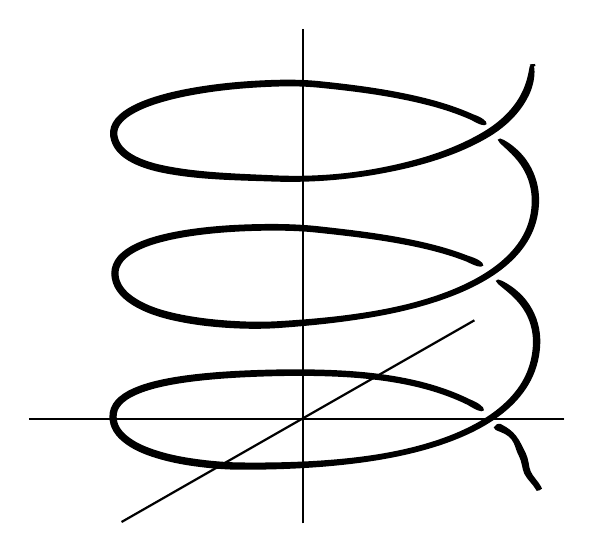
\begin{tikzpicture}[y=0.80pt, x=0.8pt,scale=0.7,yscale=-1, inner sep=0pt, outer sep=0pt]
\begin{scope}[shift={(-162.56685,-567.58888)}]% layer1
  \begin{scope}% g1809
    % path1696
    \path[draw=black,fill=black,line join=miter,line cap=butt,line width=0.800pt]
      (339.2974,567.5889) -- (339.2974,886.7834);

    % path1698
    \path[draw=black,fill=black,line join=miter,line cap=butt,line width=0.800pt]
      (508.1689,819.1861) -- (162.5668,819.1861);

    % path1700
    \path[draw=black,fill=black,line join=miter,line cap=butt,line width=0.800pt]
      (450.0975,755.7113) -- (222.4325,885.8435);

    % path1694-24
    \path[draw=black,fill=black,line join=miter,line cap=butt,line width=0.800pt]
      (464.1983,825.7867) .. controls (464.6219,826.0096) and (465.0605,826.2156) ..
      (465.5103,826.4106) .. controls (467.0261,827.0039) and (468.6894,827.6499) ..
      (470.2858,828.5303) .. controls (471.8822,829.4108) and (473.3995,830.5171) ..
      (474.5180,831.9083) .. controls (475.1923,832.7469) and (475.7200,833.6859) ..
      (476.1683,834.6622) .. controls (477.4139,837.3724) and (478.0038,840.3737) ..
      (479.4481,842.9251) .. controls (480.5316,844.8392) and (481.0096,847.0457) ..
      (481.5103,849.2110) .. controls (481.8448,851.0230) and (482.2234,852.8123) ..
      (482.9897,854.4388) .. controls (484.6982,858.0649) and (488.3433,860.9051) ..
      (490.3317,864.4338) .. controls (489.6697,865.8942) and (494.2282,863.9969) ..
      (492.5821,863.4991) .. controls (490.7602,859.9297) and (487.2857,857.0437) ..
      (485.7347,853.3748) .. controls (485.0224,851.6899) and (484.7138,849.8350) ..
      (484.4384,847.9614) .. controls (484.0129,845.7812) and (483.5855,843.5591) ..
      (482.5611,841.6104) .. controls (481.1735,838.9707) and (479.8814,836.0314) ..
      (478.2665,833.3575) .. controls (477.6887,832.3892) and (477.0637,831.4461) ..
      (476.3742,830.5727) .. controls (475.1970,829.0815) and (473.8359,827.7956) ..
      (472.3656,826.6746) .. controls (470.8953,825.5537) and (469.3206,824.5968) ..
      (467.6622,823.7569) .. controls (467.3517,823.6013) and (467.0402,823.4445) ..
      (466.7277,823.2856) .. controls (466.0189,823.0116) and (464.0487,823.1486) ..
      (463.5020,824.8466) .. controls (463.5024,825.3885) and (463.8887,825.5766) ..
      (464.1983,825.7867) -- cycle(476.3404,740.8623) .. controls
      (478.5307,743.0609) and (480.5093,745.4285) .. (482.1965,747.9945) .. controls
      (482.1965,747.9945) and (482.1965,747.9945) .. (482.1965,747.9945) .. controls
      (486.4653,754.3958) and (488.7294,762.2237) .. (488.6072,770.0698) .. controls
      (488.6072,770.0698) and (488.6072,770.0698) .. (488.6072,770.0698) .. controls
      (488.4828,777.7919) and (486.7267,785.5515) .. (483.2473,792.5272) .. controls
      (479.8256,799.4193) and (474.7750,805.5551) .. (468.8963,810.7752) .. controls
      (468.8963,810.7752) and (468.8963,810.7752) .. (468.8963,810.7752) .. controls
      (462.4316,816.5132) and (454.9850,821.1885) .. (447.1669,825.1025) .. controls
      (447.1669,825.1025) and (447.1669,825.1025) .. (447.1669,825.1025) .. controls
      (438.5041,829.4385) and (429.3629,832.8466) .. (420.0443,835.6193) .. controls
      (416.7346,836.6041) and (413.4028,837.5114) .. (410.0527,838.3456) .. controls
      (393.0095,842.5895) and (375.5085,844.9373) .. (357.9989,846.3675) .. controls
      (338.4657,847.9630) and (318.8591,848.3495) .. (299.2763,848.1409) .. controls
      (290.6947,848.0494) and (282.1250,847.3788) .. (273.6061,846.3070) .. controls
      (269.7034,845.8151) and (265.8109,845.2401) .. (261.9442,844.5480) .. controls
      (256.5902,843.5896) and (251.2939,842.3588) .. (246.1084,840.7675) .. controls
      (238.5250,838.4241) and (231.0089,835.4817) .. (225.1676,830.4508) .. controls
      (222.8961,828.4909) and (220.9165,826.2087) .. (219.7618,823.5929) .. controls
      (218.6498,821.1247) and (218.3198,818.3069) .. (218.7499,815.6384) .. controls
      (218.9685,814.2644) and (219.4968,812.9277) .. (220.2381,811.7218) .. controls
      (221.0479,810.3982) and (222.1375,809.2154) .. (223.3581,808.1466) .. controls
      (226.4243,805.4555) and (230.2500,803.6139) .. (234.2213,802.0392) .. controls
      (234.2213,802.0392) and (234.2213,802.0392) .. (234.2213,802.0392) .. controls
      (239.3164,800.0405) and (244.6659,798.6445) .. (250.0961,797.4856) .. controls
      (250.0961,797.4856) and (250.0961,797.4856) .. (250.0961,797.4856) .. controls
      (256.4764,796.1279) and (262.9482,795.1510) .. (269.4589,794.3616) .. controls
      (279.5033,793.1443) and (289.6037,792.3766) .. (299.7334,791.8475) .. controls
      (304.0788,791.6205) and (308.4296,791.4375) .. (312.7833,791.2874) .. controls
      (326.0777,790.8306) and (339.3852,790.6934) .. (352.6901,791.0547) .. controls
      (370.3638,791.5370) and (388.0549,792.9038) .. (405.4285,796.3654) .. controls
      (419.4002,799.1496) and (433.2192,803.3181) .. (446.0355,809.6376) .. controls
      (448.9772,811.4514) and (451.2070,812.6141) .. (452.7728,813.2007) .. controls
      (454.3386,813.7872) and (455.2369,813.7954) .. (455.4055,813.3585) .. controls
      (455.5741,812.9217) and (455.0076,812.0380) .. (453.6003,810.9326) .. controls
      (452.1931,809.8273) and (449.9402,808.5007) .. (446.7720,807.2831) .. controls
      (433.8560,800.9054) and (419.9861,796.6721) .. (405.9972,793.8438) .. controls
      (388.4429,790.2869) and (370.6066,788.8428) .. (352.8339,788.3010) .. controls
      (339.4554,787.8919) and (326.0780,787.9826) .. (312.7179,788.3925) .. controls
      (308.6643,788.5168) and (304.6104,788.6697) .. (300.5580,788.8599) .. controls
      (290.0408,789.3536) and (279.5337,790.0986) .. (269.0641,791.3281) .. controls
      (262.4835,792.1009) and (255.9123,793.0713) .. (249.4016,794.4338) .. controls
      (243.8671,795.5906) and (238.3466,797.0208) .. (233.0107,799.0920) .. controls
      (228.8599,800.6918) and (224.7193,802.7147) .. (221.1985,805.7492) .. controls
      (219.7810,806.9734) and (218.4816,808.4040) .. (217.4489,810.0693) .. controls
      (216.4982,811.6087) and (215.8252,813.3418) .. (215.5274,815.1759) .. controls
      (215.0005,818.4569) and (215.4130,821.8916) .. (216.7906,824.9806) .. controls
      (218.2412,828.1617) and (220.5065,830.8281) .. (223.0530,832.9867) .. controls
      (229.4850,838.4526) and (237.3875,841.6217) .. (245.1409,843.9731) .. controls
      (245.1409,843.9731) and (245.1409,843.9731) .. (245.1409,843.9731) .. controls
      (249.7013,845.3768) and (254.3298,846.5082) .. (258.9924,847.4221) .. controls
      (263.6660,848.3382) and (268.4114,849.0672) .. (273.1917,849.6603) .. controls
      (281.7375,850.7249) and (290.4649,851.3678) .. (299.2782,851.3909) .. controls
      (318.8005,851.4418) and (338.6634,850.7755) .. (358.2454,848.9604) .. controls
      (376.3933,847.2821) and (394.3699,844.6408) .. (411.3747,840.3659) .. controls
      (414.5074,839.5784) and (417.6073,838.7368) .. (420.6748,837.8382) .. controls
      (430.2298,835.0395) and (439.4823,831.6494) .. (448.2386,827.3795) .. controls
      (456.2881,823.4585) and (463.9501,818.7541) .. (470.6942,812.9289) .. controls
      (476.8640,807.6028) and (482.2172,801.2602) .. (485.9611,793.9865) .. controls
      (489.7234,786.6555) and (491.7119,778.4738) .. (491.9177,770.2148) .. controls
      (492.1284,761.7942) and (489.8017,753.2825) .. (485.1009,746.1496) .. controls
      (484.2665,744.8852) and (483.3699,743.6647) .. (482.4178,742.4863) .. controls
      (480.9928,740.7538) and (479.0100,738.7133) .. (476.8093,736.8696) .. controls
      (474.6086,735.0258) and (472.2024,733.3765) .. (470.1314,732.1894) .. controls
      (468.0604,731.0023) and (466.3372,730.2630) .. (465.4910,730.1417) .. controls
      (464.6448,730.0204) and (464.6858,730.4993) .. (465.9885,731.8935) .. controls
      (467.5535,733.2176) and (469.3679,734.6447) .. (471.1748,736.1554) .. controls
      (472.9816,737.6660) and (474.7775,739.2634) .. (476.3404,740.8623) --
      cycle(476.8581,650.3577) .. controls (478.6743,652.4066) and
      (480.3190,654.5811) .. (481.7391,656.8961) .. controls (481.7392,656.8961) and
      (481.7392,656.8961) .. (481.7392,656.8961) .. controls (485.6517,663.2014) and
      (487.7896,670.6889) .. (487.8225,678.2349) .. controls (487.8502,685.0520) and
      (486.4734,691.9278) .. (483.6160,698.1836) .. controls (480.8074,704.3652) and
      (476.5865,709.9608) .. (471.6136,714.8128) .. controls (471.6136,714.8128) and
      (471.6136,714.8128) .. (471.6136,714.8128) .. controls (466.1748,720.1170) and
      (459.8486,724.5615) .. (453.1605,728.3768) .. controls (453.1605,728.3768) and
      (453.1605,728.3768) .. (453.1605,728.3768) .. controls (445.7836,732.5837) and
      (437.9507,736.0273) .. (429.9315,738.9497) .. controls (422.6694,741.5962) and
      (415.2589,743.8279) .. (407.7552,745.7155) .. controls (397.3851,748.3242) and
      (386.8396,750.2747) .. (376.2614,751.8438) .. controls (359.2003,754.3748) and
      (342.0030,755.8409) .. (324.7950,756.9088) .. controls (314.1285,757.5707) and
      (303.4276,757.3874) .. (292.7678,756.6984) .. controls (282.1835,756.0127) and
      (271.6356,754.8188) .. (261.2587,752.7830) .. controls (260.2550,752.5861) and
      (259.2533,752.3795) .. (258.2536,752.1632) .. controls (248.5588,750.0528) and
      (238.9013,747.2062) .. (230.7460,741.8756) .. controls (227.6052,739.8179) and
      (224.7165,737.3834) .. (222.6842,734.3913) .. controls (220.8778,731.7458) and
      (219.7927,728.6063) .. (219.7576,725.4789) .. controls (219.6838,722.4136) and
      (221.0493,719.3560) .. (223.0991,716.9629) .. controls (225.6799,713.9417) and
      (229.2425,711.7661) .. (232.9884,709.9093) .. controls (232.9884,709.9093) and
      (232.9884,709.9093) .. (232.9884,709.9093) .. controls (237.8007,707.5520) and
      (242.9648,705.8785) .. (248.2330,704.4812) .. controls (248.2330,704.4812) and
      (248.2330,704.4812) .. (248.2330,704.4812) .. controls (254.4566,702.8360) and
      (260.8099,701.6429) .. (267.2151,700.6853) .. controls (278.1105,699.0577) and
      (289.1045,698.1151) .. (300.1357,697.6014) .. controls (303.4392,697.4476) and
      (306.7462,697.3323) .. (310.0548,697.2512) .. controls (323.1078,696.9362) and
      (336.1612,697.0979) .. (349.1092,698.4795) .. controls (366.6864,700.3566) and
      (384.2443,702.3240) .. (401.6256,705.4972) .. controls (416.4923,708.2122) and
      (431.3395,711.6650) .. (445.4329,717.1992) .. controls (448.4844,718.7475) and
      (450.7918,719.6896) .. (452.3907,720.1199) .. controls (453.9896,720.5503) and
      (454.8775,720.4665) .. (455.0039,720.0158) .. controls (455.1303,719.5651) and
      (454.4906,718.7464) .. (453.0070,717.7864) .. controls (451.5234,716.8265) and
      (449.1922,715.7265) .. (445.9748,714.7931) .. controls (431.8103,709.2128) and
      (416.9616,705.7022) .. (402.1576,702.9576) .. controls (384.6786,699.7068) and
      (367.0605,697.6716) .. (349.4705,695.7346) .. controls (336.3484,694.2891) and
      (323.1590,694.0735) .. (310.0142,694.3448) .. controls (306.9990,694.4068) and
      (303.9835,694.4972) .. (300.9690,694.6191) .. controls (289.5207,695.0822) and
      (278.0865,695.9999) .. (266.7315,697.6534) .. controls (260.2391,698.5985) and
      (253.7653,699.7940) .. (247.3858,701.4573) .. controls (241.9927,702.8612) and
      (236.6283,704.5929) .. (231.5369,707.0625) .. controls (227.5704,708.9708) and
      (223.6649,711.4020) .. (220.6151,714.8904) .. controls (218.0954,717.7801) and
      (216.4683,721.5611) .. (216.4946,725.5819) .. controls (216.5660,729.4133) and
      (217.8414,733.1524) .. (219.9958,736.2897) .. controls (222.3873,739.7490) and
      (225.5794,742.4853) .. (228.9658,744.6749) .. controls (228.9658,744.6749) and
      (228.9658,744.6749) .. (228.9658,744.6749) .. controls (237.6700,750.3250) and
      (247.6861,753.3378) .. (257.5355,755.4518) .. controls (257.7845,755.5059) and
      (258.0336,755.5594) .. (258.2828,755.6123) .. controls (269.3992,757.9723) and
      (280.9327,759.3158) .. (292.5877,759.9848) .. controls (303.2853,760.6029) and
      (314.1577,760.6783) .. (325.0254,759.8773) .. controls (325.0255,759.8773) and
      (325.0255,759.8773) .. (325.0255,759.8773) .. controls (342.3240,758.6015) and
      (359.6847,756.8762) .. (376.6342,754.2241) .. controls (387.6678,752.5002) and
      (398.5574,750.4056) .. (409.0747,747.7355) .. controls (416.4701,745.8579) and
      (423.6819,743.6995) .. (430.7047,741.2000) .. controls (438.9158,738.2777) and
      (446.8776,734.8563) .. (454.3951,730.6848) .. controls (454.3951,730.6848) and
      (454.3951,730.6848) .. (454.3951,730.6848) .. controls (461.2928,726.8609) and
      (467.8402,722.3693) .. (473.5627,716.9415) .. controls (478.8089,711.9680) and
      (483.3171,706.1454) .. (486.4203,699.5705) .. controls (489.5354,692.9514) and
      (491.1151,685.6502) .. (491.1495,678.3135) .. controls (491.1878,670.2394) and
      (488.9916,662.1242) .. (484.7024,655.1436) .. controls (484.1040,654.1708) and
      (483.4703,653.2206) .. (482.8040,652.2925) .. controls (481.4908,650.4969) and
      (479.6450,648.3645) .. (477.5730,646.4165) .. controls (475.5010,644.4686) and
      (473.2144,642.7041) .. (471.2311,641.4194) .. controls (469.2478,640.1348) and
      (467.5814,639.3163) .. (466.7492,639.1555) .. controls (465.9170,638.9947) and
      (465.9315,639.4732) .. (467.1410,640.9215) .. controls (468.6147,642.3126) and
      (470.3264,643.8202) .. (472.0248,645.4131) .. controls (473.7232,647.0059) and
      (475.4051,648.6867) .. (476.8581,650.3577) -- cycle(483.4485,604.1584) ..
      controls (483.2477,604.7144) and (483.0362,605.2674) .. (482.8148,605.8172) ..
      controls (480.7386,610.9714) and (477.7137,615.7940) .. (474.0361,620.1026) ..
      controls (474.0361,620.1026) and (474.0361,620.1026) .. (474.0361,620.1026) ..
      controls (468.9532,626.0674) and (462.5823,631.0283) .. (455.6373,635.0855) ..
      controls (455.6373,635.0856) and (455.6373,635.0856) .. (455.6373,635.0856) ..
      controls (436.6046,646.1929) and (414.9007,652.8263) .. (392.9614,657.2893) ..
      controls (392.9614,657.2893) and (392.9614,657.2893) .. (392.9614,657.2893) ..
      controls (385.2396,658.8597) and (377.4495,660.1353) .. (369.6167,661.0830) ..
      controls (353.2431,663.0642) and (336.6935,663.6101) .. (320.2255,662.8280) ..
      controls (320.2255,662.8280) and (320.2255,662.8280) .. (320.2255,662.8280) ..
      controls (310.1362,662.3488) and (300.0367,661.9887) .. (289.9649,661.3485) ..
      controls (289.9649,661.3485) and (289.9649,661.3485) .. (289.9649,661.3485) ..
      controls (279.0776,660.6560) and (268.2083,659.7169) .. (257.4892,657.9503) ..
      controls (257.4892,657.9503) and (257.4892,657.9503) .. (257.4891,657.9503) ..
      controls (249.9646,656.7022) and (242.4393,655.1879) .. (235.4778,652.4033) ..
      controls (233.9817,651.8049) and (232.5132,651.1426) .. (231.0787,650.4069) ..
      controls (227.9619,648.8043) and (225.0273,646.8419) .. (222.7984,644.2720) ..
      controls (220.8306,642.0112) and (219.4561,639.2223) .. (219.0581,636.3079) ..
      controls (218.8627,634.9122) and (218.9893,633.4683) .. (219.4188,632.1329) ..
      controls (219.8684,630.7101) and (220.6673,629.3789) .. (221.6360,628.1655) ..
      controls (224.1174,625.0466) and (227.6373,622.7953) .. (231.3099,620.8290) ..
      controls (236.1708,618.2534) and (241.3915,616.3492) .. (246.7142,614.7135) ..
      controls (253.0674,612.7655) and (259.5607,611.2643) .. (266.1109,610.0048) ..
      controls (266.1109,610.0048) and (266.1109,610.0048) .. (266.1109,610.0048) ..
      controls (280.6191,607.2167) and (295.3309,605.6104) .. (310.0854,604.7267) ..
      controls (310.0854,604.7267) and (310.0854,604.7267) .. (310.0854,604.7267) ..
      controls (312.0771,604.6086) and (314.0690,604.5010) .. (316.0606,604.4074) ..
      controls (327.4012,603.8745) and (338.7255,603.7923) .. (349.9553,604.9093) ..
      controls (349.9553,604.9093) and (349.9553,604.9093) .. (349.9554,604.9093) ..
      controls (367.8969,606.6931) and (385.8093,608.8498) .. (403.5004,612.3862) ..
      controls (418.8287,615.4522) and (434.1247,619.4198) .. (448.4257,625.8203) ..
      controls (451.1411,627.3925) and (453.2144,628.3489) .. (454.6702,628.7922) ..
      controls (456.1260,629.2355) and (456.9615,629.1634) .. (457.1151,628.7225) ..
      controls (457.2688,628.2815) and (456.7361,627.4703) .. (455.4277,626.5068) ..
      controls (454.1193,625.5433) and (452.0314,624.4281) .. (449.1113,623.4571) ..
      controls (434.7054,616.9862) and (419.3784,612.9433) .. (404.0875,609.8391) ..
      controls (386.2857,606.2133) and (368.2889,603.9773) .. (350.2984,602.1213) ..
      controls (350.2984,602.1213) and (350.2984,602.1213) .. (350.2984,602.1213) ..
      controls (339.1565,600.9722) and (327.9689,600.9715) .. (316.8140,601.4269) ..
      controls (314.5117,601.5209) and (312.2108,601.6343) .. (309.9125,601.7622) ..
      controls (309.9125,601.7622) and (309.9125,601.7622) .. (309.9125,601.7622) ..
      controls (295.0285,602.5895) and (280.1598,604.1545) .. (265.4657,606.9233) ..
      controls (265.4657,606.9233) and (265.4657,606.9233) .. (265.4657,606.9233) ..
      controls (258.8286,608.1736) and (252.2176,609.6814) .. (245.7146,611.6530) ..
      controls (240.2745,613.2992) and (234.8619,615.2673) .. (229.7318,617.9627) ..
      controls (225.8598,619.9709) and (221.9988,622.4969) .. (219.0311,626.1297) ..
      controls (217.8531,627.5789) and (216.8650,629.2639) .. (216.2467,631.1596) ..
      controls (215.6690,632.9733) and (215.5023,634.9064) .. (215.7666,636.8026) ..
      controls (216.2899,640.4224) and (217.9245,643.7857) .. (220.2888,646.4866) ..
      controls (222.9221,649.4752) and (226.1829,651.6983) .. (229.5457,653.4007) ..
      controls (230.4144,653.8427) and (231.2918,654.2598) .. (232.1769,654.6537) ..
      controls (239.9994,658.1354) and (248.5310,659.9271) .. (256.9749,661.2439) ..
      controls (267.7794,662.9558) and (278.8081,663.8007) .. (289.8240,664.3601) ..
      controls (299.9575,664.8764) and (310.0983,665.0972) .. (320.1402,665.4508) ..
      controls (337.2821,666.0538) and (354.3077,665.2567) .. (370.6031,663.2623) ..
      controls (378.3543,662.3137) and (385.9406,661.0994) .. (393.3891,659.6496) ..
      controls (393.3891,659.6496) and (393.3891,659.6496) .. (393.3891,659.6496) ..
      controls (404.6160,657.4742) and (415.6429,654.8013) .. (426.3200,651.2952) ..
      controls (436.9971,647.7891) and (447.3287,643.4570) .. (457.1512,637.8921) ..
      controls (464.3329,633.8249) and (471.0522,628.7283) .. (476.5597,622.3802) ..
      controls (479.8087,618.6342) and (482.6165,614.4509) .. (484.7772,609.9114) ..
      controls (485.1595,609.0880) and (485.5549,608.1524) .. (485.9292,607.1427) ..
      controls (486.6053,605.3185) and (487.2079,603.2507) .. (487.6062,601.2119) ..
      controls (488.0046,599.1732) and (488.1970,597.1676) .. (488.1969,595.4859) ..
      controls (488.1968,594.1062) and (488.0690,592.9557) .. (487.8703,592.1748) ..
      controls (487.7753,591.8012) and (487.6651,591.5205) .. (487.5482,591.3356) ..
      controls (487.4910,591.2527) and (487.4325,591.1975) .. (487.3733,591.1631) ..
      controls (487.9909,591.1107) and (488.4832,591.0695) .. (488.8244,591.0414) ..
      controls (489.1582,591.0138) and (489.3473,590.9984) .. (489.3663,590.9969) ..
      controls (489.3663,590.9969) and (489.3663,590.9969) .. (489.3663,590.9969) ..
      controls (489.3663,590.9969) and (489.3663,590.9969) .. (489.3663,590.9969) ..
      controls (489.3683,590.9967) and (489.3683,590.9967) .. (489.3663,590.9969) ..
      controls (489.3663,590.9969) and (489.3663,590.9969) .. (489.3663,590.9969) ..
      controls (489.3663,590.9969) and (489.3663,590.9969) .. (489.3663,590.9969) ..
      controls (489.3663,590.9969) and (489.3663,590.9969) .. (489.3663,590.9969) ..
      controls (489.3663,590.9969) and (489.3663,590.9969) .. (489.3663,590.9969) ..
      controls (489.3663,590.9969) and (489.3663,590.9969) .. (489.3663,590.9969) ..
      controls (489.3663,590.9969) and (489.3663,590.9969) .. (489.3663,590.9969) ..
      controls (489.3663,590.9969) and (489.3663,590.9969) .. (489.3663,590.9969) ..
      controls (489.3474,590.9989) and (489.1596,591.0136) .. (488.7768,591.0434) ..
      controls (488.3941,591.0732) and (487.8165,591.1178) .. (487.0167,591.1781) ..
      controls (486.9608,591.2134) and (486.9043,591.2649) .. (486.8466,591.3430) ..
      controls (486.7379,591.5133) and (486.6244,591.7647) .. (486.4976,592.1270) ..
      controls (486.4565,592.2443) and (486.4140,592.3716) .. (486.3696,592.5092) ..
      controls (486.2236,593.3375) and (486.0614,594.2260) .. (485.8802,595.1637) ..
      controls (485.5992,596.6181) and (485.2677,598.1502) .. (484.8632,599.6783) ..
      controls (484.4587,601.2064) and (483.9817,602.7300) .. (483.4485,604.1584) --
      cycle;

  \end{scope}
\end{scope}


\end{tikzpicture}
\end{center}
\end{frame}
%%%%%%next-slide%%%%%
\begin{frame}

\begin{lemat}
Niech $\alpha\colon (a,b)\to \R^3$ oraz $\overline{\alpha}\colon (c,d)\to \R^3$ będą krzywymi różnowartościowymi o tym samym obrazie. Wówczas istnieje taki dyfeomorfizm \[h\colon (a,b)\to (c,d),\] że $\overline{\alpha}$ jest reparametryzacją krzywej $\alpha$ przez $h$.
\end{lemat}
\pause \textcolor{ared}{\textbf{Dowód:}}\\
Niech $h(t)$ oznacza złożenie \[\alpha^{-1}\circ \overline{\alpha} (t)\] ($\alpha^{-1}\colon \alpha(a,b)\to \R^3$ istnieje ponieważ $\alpha$ jest r\'ożnowartościowa). Dokładne sprawdzenie że jest to szukana reparametryzacja jest zadaniem domowym.
\hfill $\square$

\end{frame}
%%%%%%next-slide%%%%%
\begin{frame}
\begin{lemat}
Niech $\alpha\colon(a,b)\to \R^3$ będzie krzywą gładką. Jeśli $\overline{\alpha}\colon (c,d)\to \R^3$ jest jej reparametryzacją, wówczas \[L(\overline{\alpha})=L(\alpha).\]
\end{lemat}

\pause \textcolor{ared}{\textbf{Dowód:}}\\
Ponieważ $\overline{\alpha}$ jest reparametryzacją $\alpha$, zatem z definicji, istnieje taki dyfeomorfizm $h\colon (c,d)\to (a,b)$, że \[\overline{\alpha}=\alpha\circ h.\] \pause Ponieważ $h$ jest dyfeomorfizmem, więc jego pochodna nie może zmieniać znaku.  Możemy bez straty ogólności przyjąć, że $h'(t)\geqslant 0$ (tj. $h$ jest funkcją niemalejącą), oraz \[h(c)=a\qquad \text{i}\qquad h(d)=b.\]
\end{frame}
%%%%%%next-slide%%%%%
\begin{frame}[<+->]
Stosując podstawienie $t=h(s)$ i $dt=h'(s)\,ds$ otrzymujemy następującą równość:\pause 
\begin{multline*}
L(\overline{\alpha})=\int_c^d\|\overline{\alpha}'(s)\|\,ds=\int_c^d\|\alpha'(h(s))h'(s)\|\,ds=\\
\pause=\int_c^d\|\alpha'(h(s))\|h'(s)\,ds=\int_{h(c)}^{h(d)}\|\alpha'(t)\|\, dt=\\
\pause=\int_{a}^{b}\|\alpha'(t)\|\, dt=L(\alpha).
\end{multline*}
\hfill $\square$

\end{frame}

\mode<all> 
